\documentclass[table]{article}
\usepackage{authblk}
\usepackage{booktabs}
\usepackage{amsmath}
\usepackage{amssymb}
\usepackage{pgfplots}  
\usepackage{todonotes}
\usepackage[hyphens]{url}
% \usepackage{colortbl}
\PassOptionsToPackage{table}{xcolor}
\pgfplotsset{compat=1.9}
\usepackage{caption}
\usepackage{subcaption}
\providecommand{\keywords}[1]{\textbf{\textit{Index terms---}} #1}
% \definecolor{col1}{HTML}{ff595e}
% \definecolor{col2}{HTML}{ffca3a}
% \definecolor{col3}{HTML}{8ac926}
% \definecolor{col4}{HTML}{1982c4}
% \definecolor{col5}{HTML}{6a4c93}

\definecolor{col1}{HTML}{ef476f}
\definecolor{col2}{HTML}{118ab2}
\definecolor{col3}{HTML}{ffd166}
\definecolor{col4}{HTML}{06d6a0}
\definecolor{col5}{HTML}{073b4c}

\newcommand{\mybox}[2]{\fcolorbox{#1}{#1!10}{#2}}



\author[1,2]{Constantinos Patsakis}
\author[2,3]{Nikolaos Lykousas}


\affil[1]{Department of Informatics, University of Piraeus, 80 Karaoli \& Dimitriou str., 18534 Piraeus, Greece}
\affil[2]{Information Management Systems Institute of Athena Research Centre, Greece}
\affil[3]{Data Centric Services, Bucharest, Romania}
% \affil[3]{Data Centric}
% Language setting
% Replace `english' with e.g. `spanish' to change the document language
\usepackage[english]{babel}

% Set page size and margins
% Replace `letterpaper' with `a4paper' for UK/EU standard size
\usepackage[letterpaper,top=2cm,bottom=2cm,left=3cm,right=3cm,marginparwidth=1.75cm]{geometry}

% Useful packages
\usepackage{amsmath}
\usepackage{graphicx}
\usepackage[colorlinks=true, allcolors=blue]{hyperref}

\title{Man vs the machine: The Struggle for Effective Text Anonymisation in the Age of Large Language Models}

\begin{document}
\date{}
\maketitle

\begin{abstract}
The collection and use of personal data are becoming more common in today's data-driven culture. While there are many advantages to this, including better decision-making and service delivery, it also poses significant ethical issues around confidentiality and privacy. Text anonymisation tries to prune and/or mask identifiable information from a text while keeping the remaining content intact to alleviate privacy concerns. Text anonymisation is especially important in industries like healthcare, law, as well as research, where sensitive and personal information is collected, processed, and exchanged under high legal and ethical standards.

Although text anonymization is widely adopted in practice, it continues to face considerable challenges. The most significant challenge is striking a balance between removing information to protect individuals' privacy while maintaining the text's usability for future purposes. The question is whether these anonymisation methods sufficiently reduce the risk of re-identification, in which an individual can be identified based on the remaining information in the text.

In this work, we challenge the effectiveness of these methods and how we perceive identifiers. We assess the efficacy of these methods against the elephant in the room, the use of AI over big data. While most of the research is focused on identifying and removing personal information, there is limited discussion on whether the remaining information is sufficient to deanonymise individuals and, more precisely, who can do it. To this end, we conduct an experiment using GPT over anonymised texts of famous people to determine whether such trained networks can deanonymise them. The latter allows us to revise these methods and introduce a novel methodology that employs Large Language Models to improve the anonymity of texts.



\end{abstract}
\keywords{Privacy, LLMs, text anonymisation, deanonymisation}
\section{Introduction}

In today's data-driven society, the collection and use of personal information are becoming increasingly prevalent. While this has numerous benefits, such as improved decision-making and better service provision, it also raises important ethical concerns related to privacy and confidentiality. Indeed, harvesting user data is a common practice of far too many online platforms and services with a significant impact on citizens. This has been one of the pillars that led to the introduction of the General Data Protection Regulation (GDPR) \cite{gdpr} and other relevant legislation around the world as a means to address the privacy issues that emerged. The GDPR mandates using privacy-preserving methods and processes throughout the data management lifecycle, from collection and processing to sharing and publishing. One of the fundamental such methods is anonymisation. Given that modern organisations continuously deal with documents, the above has served as a catalyst in the emergence of text anonymisation as a research topic with many practical applications. The general concept is that given a text, one has to remove or mask identifiable information  while preserving the remaining content. Text anonymisation is particularly relevant in healthcare, law, and research, where personal and sensitive information is overwhelming and must be protected to comply with privacy regulations and ethical guidelines.

Although text anonymisation has been widely adopted in practice, it still faces significant challenges. These methods must strike a balance between the need to protect the privacy of individuals and the need to preserve the data utility. Let us consider this with an example where the anonymisation task is to anonymise the sentence ``\textit{Volodymyr Zelenskyy is the president of Ukraine}''. Clearly, simply removing the name is not enough. If one is given the sentence ``\textit{\mybox{red}{NAME} is the president of Ukraine}'', it is trivial to recover the missing information. Therefore, the anonymised sentence would be ``\textit{\mybox{red}{NAME} is the president of \mybox{red}{COUNTRY}}''. To this end, named entity recognition methods are used to identify possible identifying information, such as names and locations, to mask them. Let us go back to the example. 

While the sentence is anonymised, it is easy to understand that the anonymity of the masked person is bounded. Given that the sentence refers to a country's president, there are 193 possible choices, which in terms of k-anonymity \cite{samaratiyprotecting} would be perfect. Nevertheless, even fragments of information from other sentences in the context of a text could significantly limit the possible choices. Therefore, the challenge is not only whether an algorithm finds clearly identifiable information but whether the remaining information is enough to deanonymise an individual and reveal the rest of the pruned information. For instance, using non-identifying information, e.g., referring to his acting career or studies, can limit the candidates to just a handful of people. Therefore, the challenge comes down to how much information is available and whether this can be properly extracted to infer the identity of individuals. 


In the past two years, endless discussions have sparked with the introduction of GPT from OpenAI, which boomed with the introduction of ChatGPT. The GPT-3 model was trained on a text dataset of more than 8 million documents and over 10 billion words and is 175 billion parameters in size. This allows it to perform many text-generative tasks efficiently, astonishing people worldwide. Based on the above, a natural research question is to ponder whether such systems, trained over texts with sensitive content that are available from one organisation, would be able to deanonymise published anonymised texts from another organisation. Evidently, the latter could have a catastrophic impact on individuals, despite applying best practices from the publishing organisation.


We performed a scoped experiment using GPT targeting famous individuals to assess this threat scenario. Since efficiently and effectively training such systems is by itself a challenge, we opted to use the available closed but off-the-shelf GPT to deanonymise texts that had been anonymised by a state of the art algorithm, namely Textwash \cite{kleinberg2022textwash}. The choice of testing on deanonymising famous people is that this maximises the chances of GPT to have been trained on relevant documents and that, this way, we depend solely on public information. Then, we use GPT to improve text anonymisation, increasing the actual anonymity of the texts without significantly impacting their quality.

The rest of this work is structured as follows. The next section provides an overview of the current state of the art. Then, in Section 3, we detail our threat scenario. Section 4 introduces the dataset and our methodology. Next, Section 5 presents the results of our experiments. Finally, the article concludes by discussing our findings and ideas for future work.

\section{Related work}
In the next paragraphs, we discuss personal data and identifiers. Then, we provide an overview of text anonymisation algorithms. Finally, we describe two essential parts of our work, Textwash, an open source text anonymisation tool, and the GPT model. 


% Important Points from \cite{lukas2023analyzing}:

% Existing work focuses on finding a lower bound on any kind of memorization but does not differentiate public and private leaked information. For example, leaking (highly duplicated) common phrases is not a privacy violation according to the GDPR [15] as opposed to leaking Personally Identifiable Information (PII). In practice, any LM trained on real, sensitive data has to protect PII, but memorization (specifically) of PII is not well understood. We believe that a comprehensive study on the risk of PII memorization in LMs trained on sensitive datasets is missing.
% ---- Probaby their strongest point. We don't talk about memorization or specific LM attacks at all...
% Nevertheless, I think we are the only ones talking about the feasibility of text anonymisation. lukas2023analyzing try to extract PII from the LLM-generated text, using targeted prompts. Our Threat scenario is different.

% Scrubbing techniques reduce but do not prevent the risk of PII leakage:
% in practice scrubbing is imperfect and must balance the trade-off between minimizing disclosure and preserving the utility of the dataset.
% ---- Shouldn't we say something regarding this in our threat scenario ? Why would both organizations A, B fine-tune LLMs on sensitive information without trying to anonymise it first somehow ? A reviewer might raise this question.

% The data independence of Differential Privacy can also be a limitation e.g., when sensitive content is shared within groups of users of unknown size. In these cases, the sensitive nature of the content is defined by its context and cannot be represented by an adjacency relation between pairs of datasets as pointed out by Brown et al \cite{brown2022does}. 
% ---- This is very relevant for our Threat Scenario


% In practice, training NER models is challenging because defining what constitutes PII can
% change over time and is dependent on the surrounding context \cite{brown2022does}. Moreover, (i) training NER requires domainspecific, labelled training data, (ii) NER models make errors
% (i.e. a subset of PII remain unrecognized), and (iii) existing, publicly available NER models only aim for deidentification but not anonymization \cite{pilantext}. This means that
% complex PII, whose detection requires natural language understanding such as a description of a person’s appearance, is not tagged by any publicly available NER.
% --- Isn't this closely related to the context of PSI we talk about in this paper (also introduced by Textwash ?).


\subsection{Personal data}
Personally Identifiable Information (PII) refers to any piece of information that can directly or indirectly identify a specific individual. In this regard, direct identifiers can provide an explicit link to an individual and identify them. In most cases, direct identifiers are unique values. Typical examples of direct identifiers are identity, passport, driver's license, and Social Security numbers. The name is also a direct identifier, however, they are not unique. Quasi-identifiers are attributes that do not uniquely identify individuals on their own; nevertheless, once someone combines them with other quasi-identifiers or other data, they can narrow down the possible individuals to the point of uniquely identifying the individual. Typical quasi-identifiers are birthday, gender, ethnicity, postal code, and occupation. Some legal frameworks, such as the Health Insurance Portability and Accountability Act (HIPAA) in the United States tried to define some quasi-identifiers in medical documents that have to be removed to protect the privacy of individuals. Nevertheless, as outlined by Narayanan and Shmatikov "\textit{any attribute can be identifying in combination with others}" \cite{narayanan2010myths} so subsequent legislations do not directly refer to specific identifiers and regulators acknowledge the challenges that data anonymisation faces, as well as its limitations and possible ephemeral nature\footnote{\url{https://edps.europa.eu/system/files/2021-04/21-04-27_aepd-edps_anonymisation_en_5.pdf}}.

Due to the wide harvesting and exploitation of PII by organisations worldwide, data protection and privacy regulations, such as the General Data Protection Regulation (GDPR) in the European Union and the California Consumer Privacy Act (CCPA) in the United States 

According to the GDPR (Article 4), personal data are defined as follows \cite{gdpr}:

\begin{quote}
``Personal data'' means any information relating to an identified or identifiable natural person (``data subject''); an identifiable natural person is one who can be identified, directly or indirectly, in particular by reference to an identifier such as a name, an identification number, location data, an online identifier or to one or more factors specific to the physical, physiological, genetic, mental, economic, cultural or social identity of that natural person;
\end{quote}
Therefore, the GDPR considers that personal data are pieces of information that individually or with other information can be used to identify, contact, or locate an individual. As a result, personal data are widely described as Personally Identifiable Information (PII). Due to the sensitivity of the underlying data, data protection and privacy regulations, such as the General Data Protection Regulation (GDPR) in the European Union or the California Consumer Privacy Act (CCPA) in the United States make specific provisions on the collection, handling, and management of such data. As a result, organisations must adopt appropriate data protection techniques, such as anonymisation, pseudonymisation, or encryption, subject to constraints on the type and volume of data, user roles, and jurisdiction, to name a few. They should also follow the principles of data minimisation and privacy by design, which means collecting and processing only the necessary data and incorporating privacy considerations from the outset of any project. Of specific interest is consent management, as organisations are obliged to have the direct and informed consent of the data subjects to collect and process their data. Nevertheless, the aggregated and anonymised version of user data can be published without their consent, as theoretically, the identifying information has been removed and individuals cannot be identified. Indeed, according to the GDPR: ``\textit{This Regulation does not therefore concern the processing of such anonymous information, including for statistical or research purposes}".


\subsection{Data anonymisation methods}
To anonymise data there are various methods that depend on the underlying information and how it would be published. For instance, there are specific methods for tabular data which may greatly vary depending on whether an updated version of the dataset would have to be published again. Such methods may generalise or suppress records, introduce noise, slice the data etc. \cite{zigomitros2020survey}. Nevertheless, such data are well-defined and have very specific and structured information. Similarly, transactional and trajectory data may have to employ similar methods, e.g. noise addition and generalisation, yet in different contexts to make the data reusable.

However, for textual data, the approaches are radically different as information is not well structured, at least for a machine. Therefore, the first step to applying a text anonymisation algorithm is to identify the structure of the document that would allow one to trace potentially sensitive information and then prioritise these pieces of  information, e.g., to purge the ones that seem more appropriate. Apparently, the above describes a natural language processing task, and named entity recognition plays a central role \cite{mamede2016automated,978-3-030-00202-2_24,kleinberg2017netanos}. 

While mainly dictionary and pattern-based, Scrub \cite{sweeney1996replacing} was the first such method and targeted the anonymisation of medical records. Neamatullah et al. \cite{neamatullah2008automated} followed the same path as their approach is also based on dictionaries, however, they use regular expressions and simple heuristics to locate possible sensitive information, including doctor names and years of dates. Similarly, Ruch et al.  \cite{ruch2000medical} utilised semantic lexicon to anonymise medical documents. Dernoncourt et al. \cite{dernoncourt2017identification} used a long short-term memory (LSTM) to anonymise patient notes that were tokenised text using the Stanford
CoreNLP tokeniser \cite{manning2014stanford}. LSTMs alongside conditional random field (CRF) and regular expressions were also utilised in \cite{LIU2017S34} to anonymise clinical notes. S{\'a}nchez et al. \cite{sanchez2012detecting,6410029,sanchez2014utility} leverage Information Content, disclosure risk, and knowledge bases to detect possible sensitive content in tokenised texts. Uzuner et al. \cite{UZUNER200813} introduced Stat De-id which uses support vector machines to anonymise medical discharge summaries by assessing whether each word in the text is a sensitive feature.

For more details, the interested reader may refer to \cite{meystre2010automatic,lison2021anonymisation}.




\subsection{Textwash}
One of the latest tools for text anonymisation is Textwash \cite{kleinberg2022textwash}, an open-source tool introduced by Kleinberg et al., specifically addressing the problem of privacy-preserving data sharing.
The general concept of Textwash is to identify sensitive and potentially sensitive information and redact it while maintaining semantic coherence to ensure that the anonymised out remains usable
for various downstream text analysis tasks.%followed by a numeric identifier to enable semantic coherence. 
Textwash is based on supervised machine learning, leveraging pre-trained contextualised word representations provided by a fine-tuned BERT language model. Much like the NER-based text anonymisation tools, the categories of redactable text data considered by Textwash comprise a pre-defined set of 11 possible tags, the annotations provided by domain experts. 
More precisely, the possible tags are PERSON\_FIRSTNAME, PERSON\_LASTNAME, OCCUPATION, LOCATION, TIME, ORGANIZATION, DATE, ADDRESS, PHONE\_NUMBER, EMAIL\_ADDRESS, and OTHER\_IDENTIFYING\_ATTRIBUTE.
The last tag comprises a meta-category which encapsulates the \textbf{potentially sensitive information} (PSI) concept. Concretely, the PSI notion captures the full spectrum of textual information that could reveal an identity which cannot be attributed to a well-defined category of PII. This is made possible by leveraging the contextual awareness of its Transformer-based architecture \cite{DevlinCLT19,liu2019roberta,xia2020bert}.

To preserve the semantic properties of anonymised texts while removing any identifiable information, Textwash implements a two-stage anonymisation process. Specifically, after a token is classified as one of the 11 possible categories (e.g. John), it will be replaced with the relevant tag (e.g. \mybox{red}{PERSON\_FIRSTNAME}), with a numeric suffix incremented for each different instance of the specific category. For instance, if in the document there is another name, e.g. George, then each occurrence of John would be replaced by \mybox{red}{PERSON\_FIRSTNAME\_1}, and each occurrence of George would be replaced by \mybox{red}{PERSON\_FIRSTNAME\_2}.
% actually this part is not related to the underlying BERT
% To achieve this, Textwash uses BERT \cite{DevlinCLT19} trained with various annotated public text sources from two experts that allow it to create contextualised word representations. 



%Thus, the possible tags are PERSON\_FIRSTNAME, PERSON\_LASTNAME, OCCUPATION, LOCATION, TIME, ORGANIZATION, DATE, ADDRESS, PHONE\_NUMBER, EMAIL\_ADDRESS, and OTHER\_IDENTIFYING\_ATTRIBUTE. Once Textwash finds a name, e.g. John, it will replace it with PERSON\_FIRSTNAME in every occurrence. However, if in the document there is another name, e.g. George, then each occurrence of John would be replaced by PERSON\_FIRSTNAME\_1, and each occurrence of George would be replaced by PERSON\_FIRSTNAME\_2. To achieve this, Textwash uses BERT \cite{DevlinCLT19} trained with various annotated public text sources from two experts that allow it to create contextualised word representations. The latter enables Textwash to accurately predict whether individual words and phrases contain sensitive information. 


\subsection{GPT}

GPT-3 is a large language model (LLM) \cite{brants2007large} that relies on techniques such as tokenisation, part-of-speech tagging, named entity recognition, and syntactic parsing to understand the structure and meaning of natural language text. The underlying architecture of GPT-3 is based on the transformer model \cite{vaswani2007attention}, which is highly effective for natural language processing tasks. According to OpenAI, the training data for GPT-3 includes various sources such as books, articles, and websites, with a primary source being the Common Crawl\footnote{\url{https://commoncrawl.org/}}, a repository of web pages and documents that is regularly updated and maintained and its training process is described in \cite{brown2020language}. Currently, GPT-3 is also used in various practical applications, including chatbots, with ChatGPT being in the spotlight, language translation, and text completion. 

However, GPT-3 and other AI models also raise ethical concerns. There has been a growing body of research on topics such as fairness, accountability, and transparency in AI to ensure that models are developed and deployed in an ethical and transparent manner. For instance, given the increasing role of AI, negligence and liability \cite{selbst2020negligence,smith2020artificial} must be reconsidered. The above concerns led Brundage et al. \cite{brundage2020toward} to propose ways to ensure that AI models are developed and deployed ethically and transparently and the EU Commission to push towards the development of the AI Act \cite{aiact}, the first law on AI by a major regulator anywhere in the world, to mitigate possible risks from the wrong use of AI and regulate its development and deployment in a well-defined legal and regulatory framework.


\section{Threat scenario}\label{sec:scenario}
% One of the crucial questions is the feasibility of the attack scenario. 
Currently, GitHub's Copilot\footnote{\url{https://github.com/features/copilot}} uses OpenAI's Codex\footnote{\url{https://openai.com/blog/openai-codex/}} a descendant of GPT-3, as it is based both on a corpus from both physical language and code documents. Interestingly, Copilot was reportedly leaking secrets and only recently did GitHub issue measures to stop it from doing so\footnote{\url{https://www.bleepingcomputer.com/news/security/github-copilot-update-stops-ai-model-from-revealing-secrets/}}. The above means that LLMs can now efficiently understand sensitive information and its context. Therefore, we face the following threat. If an LLM is trained on a large corpus of sensitive information, then it may have the capacity to deanonymise relevant anonymised texts. By merely removing obviously sensitive parts, we cannot guarantee that the result would provide the privacy guarantees that we would expect. Due to the continuous increase in the quality and size of training datasets, as well as the sophistication to calibrate them, LLMs are managing to perform many tasks with high efficiency. Therefore, we must also consider them part of the attack tooling. Given the sear amount of data that modern organisations hold, it is only a matter of time until some of them try to feed this data to such systems. Going back to the Copilot use case, where secrets were leaked when one had to fill in a password, we can assume that these LLMs could fill in the gaps of missing information, including the case of anonymised texts.

Based on the above, we consider the following threat scenario. 
Let there be two organisations $\mathcal{A}$ and $\mathcal{B}$ having two text datasets $T_\mathcal{A}$ and $T_\mathcal{B}$, respectively. These sets refer to their clients, denoted as $C_\mathcal{A}$ and $C_\mathcal{B}$, respectively and $C_\mathcal{A}\cap C_\mathcal{B}\neq\emptyset$. The two organisations exchange information as a basis of their collaboration, but due to legal and regulatory constraints; they anonymise them. Therefore, having in hand two anonymisation functions $Anon_1$ and $Anon_2$ (not necessarily the same), they send to each other $Anon_1(T_\mathcal{A})$ and $Anon_2(T_\mathcal{B})$. Setting aside the legal and ethical constraints, $\mathcal{A}$ trains/fine-tunes (depending on its capacity) $LLM_\mathcal{A}$ with $T_\mathcal{A}$. Our new threat scenario considers the exposure of $C_\mathcal{B}$ from the use of $LLM_\mathcal{A}$ on $Anon_2(T_\mathcal{B})$ that $\mathcal{A}$ receives from $\mathcal{B}$. In what follows, we consider that $Anon_2$ is a black box; however, further tuning could be performed knowing how it works.




\section{Dataset and methodology}
In our experiments, we use the dataset from \cite{kleinberg2022textwash}. More precisely, we use the data from the second study of Kleinberg et al., which contains 1080 descriptions of 20 famous individuals in the UK and their anonymised versions. Kleinberg et al. assigned 200 participants to write a description of some random subset of these celebrities in English. As a result, for each individual, there are 46 to 61 descriptions, with an average of 54. Then, these descriptions were anonymised by Textwash.  
The text in Figure \ref{fig:jagger} is a sample anonymised text from this dataset. Afterwards, Kleinberg et al. recruited 222 participants to deanonymise ten random texts from this dataset and recorded their success rate. By using this dataset, we refrain from processing any private information, as the whole dataset consists of information about famous individuals such as Adele, David Beckham, and Luis Hamilton, and the information is provided by individuals who have no relation to them. Therefore, the information is not sensitive, it is public, and the data subjects have chosen to make it public. Moreover, due to the fact that they are celebrities, it is highly possible that GPT has already been trained on documents containing related information. Clearly, the relevant documents that might have been used for the training of GPT are different from those used in the dataset.

\begin{figure}
    \centering
\noindent\fbox{%
    \parbox{\textwidth}{
\mybox{red}{PERSON\_FIRSTNAME\_2} \mybox{red}{PERSON\_LASTNAME\_1} is an \mybox{red}{LOCATION\_1} singer, songwriter, actor and film producer who was born on \mybox{red}{DATE\_1} \mybox{red}{DATE\_1} \mybox{red}{DATE\_1} and is now \mybox{red}{NUMERIC\_1} years old. \mybox{red}{PERSON\_FIRSTNAME\_2} \mybox{red}{PERSON\_LASTNAME\_1} is the lead singer of rock band, \mybox{red}{ORGANIZATION\_2}. \mybox{red}{PERSON\_FIRSTNAME\_2} \mybox{red}{PERSON\_LASTNAME\_1} is known as a rock legend and for \mybox{red}{PRONOUN} charismatic stage presence and dancing. So much so, that \mybox{red}{ORGANIZATION\_1} released a song after \mybox{red}{PRONOUN} dancing, called \mybox{red}{OTHER\_IDENTIFYING\_ATTRIBUTE\_1} like \mybox{red}{PERSON\_LASTNAME\_1}'. \mybox{red}{PERSON\_FIRSTNAME\_2} \mybox{red}{PERSON\_LASTNAME\_3} has \mybox{red}{NUMERIC\_4} children, and has had multiple partners, and \mybox{red}{NUMERIC\_1} spouse. \mybox{red}{PERSON\_FIRSTNAME\_2} \mybox{red}{PERSON\_LASTNAME\_1} has been with \mybox{red}{PRONOUN} current partner \mybox{red}{PERSON\_FIRSTNAME\_1} \mybox{red}{PERSON\_LASTNAME\_2} since \mybox{red}{DATE\_2}.
}%
}
\caption{An anonymised version of the text for Mick Jagger in the dataset.}
    \label{fig:jagger}
\end{figure}

Using this dataset, we aim to assess whether the anonymised version can lead to the deanonymisation of a document using an LLM. According to OpenAI, GPT-3 does not use online information; therefore, all its responses are based on what the model has learned through its training. Indeed, OpenAI in its ``API data usage policies'' states:
\begin{quote}
    \textit{OpenAI will not use data submitted by customers via our API to train or improve our models, unless you explicitly decide to share your data with us for this purpose.}\footnote{\url{https://openai.com/policies/api-data-usage-policies}}
\end{quote}
Therefore, the information that we used in our experiments was not used to retrain the model.

Having the above dataset at hand, we created a set of tasks for GPT-3, asking it to guess the name of the person that would fit most to each of the provided anonymised descriptions. This is illustrated in Figure \ref{fig:deanon}.
\begin{figure}[th]
    \centering
    \includegraphics[width=\textwidth]{images/deanonymisation.png}
    \caption{Deanonymisation methodology}
    \label{fig:deanon}
\end{figure}

The results; discussed in the following section, led us to consider the revision of text anonymisation algorithms. We argue that the existence of LLMs and their ability to extract knowledge from large quantities of text, in conjunction with their zero-shot reasoning capacity, offer advanced features for text anonymisation. Therefore, we consider a revised text anonymisation methodology, as illustrated in Figure \ref{fig:anon}. Practically, an LLM is queried to report which pieces of identifying information should be pruned. Then, we remove these pieces of information from each text, leading to an improved anonymised version of the dataset. While some records could still be identified,  since the adversary would not have access to the same dataset to train the LLM, the risk exposure would be significantly less than in our experiments. 

\begin{figure}[th]
    \centering
    \includegraphics[width=\textwidth]{images/anonymisation.png}
    \caption{Proposed anonymisation methodology}
    \label{fig:anon}
\end{figure}

\section{Experimental results}
In what follows, we detail our two experiments and their results, illustrated in Figure \ref{fig:exp_flow}.
\subsection{Deanonymisation}
The first experiment is a `motivated intruder' test, focused on a zero-shot deanonymisation task. Concretely, we attempt to replicate the deanonymisation task presented in \cite{kleinberg2022textwash}, but we modify the experiment by substituting Prolific Academic participants with an LLM. In this context, we used the 1080 anonymised descriptions of the 20 celebrities and assigned GPT to guess the person this information refers to. To reduce the noise in the input, before submitting each text, we used a regular expression to remove any tags that were inserted by Textwash, e.g. PERSON\_FIRSTNAME\_1, PRONOUN, DATE, etc. Specifically, we evaluated the most recent iteration of GPT-3 models provided by OpenAI, namely \texttt{text-davinci-003} and \texttt{gpt-3.5-turbo}, both being part of ``GPT-3.5'' series\footnote{At the time of writing, the next iteration of GPT, namely GPT-4, is in a limited beta with not generally available.}. At the time of writing, contrary to previous GPT versions, these recent models based on reinforcement learning from human feedback (RLHF)\cite{ouyang2022training}, do not support fine-tuning using the OpenAI API. In order to establish which one of these pre-trained LLMs performed best for this task, we randomly sampled 100 anonymised person descriptions from the dataset and tried different prompts replicating the motivated intruder task of identifying the described person. In our trials, the latest \texttt{gpt-3.5-turbo} model consistently performed better than \texttt{text-davinci-003}, by a margin of 25-30\%. Moreover, we observed that for the first model, syntactic differences in prompts describing the task had negligible impact on the model's accuracy. As such, henceforth we run every experiment using the \texttt{gpt-3.5-turbo} model. The prompt template we used for this experiment is shown in \ref{prompt:intruder}.

\begin{figure}[th]
    \centering
    \includegraphics[width=\textwidth]{images/experimental.png}
    \caption{The data flow of the two experiments.}
    \label{fig:exp_flow}
\end{figure}


In total, GPT deanonymised 784 texts correctly, which is 72.6\% of the total. Notably, the humans in the original experiments of Kleinberg et al. \cite{kleinberg2022textwash} deanonymised 285 texts, which is 26.39\% of the total. Practically, using an LLM such as GPT the deanonymisation almost tripled since the correctly anonymised texts were 2.75 times the ones that humans anonymised. As it can be observed in Figure \ref{fig:anon_exp}, the results are consistent. For every celebrity, GPT clearly outperforms humans in the motivated intruder test. Notably, in terms of percentages, the closest result was for D. Beckham (166\% better), and the biggest difference was for D. Radcliffe (almost eight times better). 

Beyond the outstanding results in deanonymisation, of specific interest are the misclassifications, illustrated in Figure \ref{fig:misclass}. On the left hand side with blue colour, we have the 20 celebrities from the original dataset, and on the right hand side and in red, we have all the recorded misclassifications. The most often misclassifications are of J. Dench with M. Streep and D. Radcliffe with D. Craig. Nevertheless, for most of the misclassification, there are well-justified arguments why these two celebrities could be mixed with each other. Of specific interest was that in our initial experiments, we noticed several misclassifications between JK Rowling and Sam Smith. Given that they both belong to the dataset, the excellent performance of GPT in the task, and that the link between them is not direct, we decided to inspect the relevant texts. Interestingly, we noticed that the dataset providers wrongly classified eight texts in the dataset; they were attributed to JK Rowling while the text was actually describing Sam Smith and vice versa\footnote{\url{https://github.com/maximilianmozes/textwash/blob/d347f40cab948bdcb522e3f8829c2a9b05bd7fbc/paper/study2/person_descriptions/orig/rowling_69.txt}}. The latter perfectly exhibits the prevalence of the deanonymisation attack and the risk from this attack vector.

Finally, we asked GPT again for a second guess for the misclassified celebrities, and 77 more were correctly identified, reaching a correct deanonymisation of 79.72\%. Since there is no similar result for humans, we cannot have a fair comparison. Yet, it illustrates that there is potential for further improvements as, e.g. confidence levels for each response can be provided for each response.


\begin{table}[th]
    \centering
    \begin{subtable}[h]{0.33\textwidth}
        \centering
        \begin{tabular}{|p{.9\textwidth}|}
            \hline
            \cellcolor{col2!10}\textbf{System:} You are very knowledgeable about celebrities. When asked to identify individuals, disregard any missing information and context, and respond only with the name within quotes of the most likely celebrity candidate being referred to in the provided text.\\   
            \hline \textbf{User:} Identify the person: \mybox{col2}{[TEXT]}\\
           % \hline \cellcolor{col2!10}\textbf{Assistant:} "PERSON"\\
            \hline
        \end{tabular}
        \caption{Motivated intruder test}
        \label{prompt:intruder}
    \end{subtable}~
        \begin{subtable}[h]{0.33\textwidth}
        \centering
        \begin{tabular}{|p{.9\textwidth}|}
            \hline
            \cellcolor{col2!10}\textbf{System:} You are an efficient assistant. Keep your responses short and provide no explanations.\\   
            \hline \textbf{User:} Anonymise and remove any personally identifiable information and related context from the given text: \mybox{col2}{[TEXT]}\\
           % \hline \cellcolor{col2!10}\textbf{Assistant:} "PERSON"\\
            \hline
        \end{tabular}
        \caption{Anonymisation}
        \label{prompt:anon}
    \end{subtable}~
        \begin{subtable}[h]{0.33\textwidth}
        \centering
        \begin{tabular}{|p{.9\textwidth}|}
            \hline
            \cellcolor{col2!10}\textbf{System:} You are an efficient assistant. Keep your responses short and provide no explanations.\\   
            \hline \textbf{User:} Identify every token (including words, dates, and numerals) in the provided person description that can be connected to the person being talked about, such that if these tokens are removed the resulting text is anonymised. Return these words as a JSON-formatted list. The description of this person is: \mybox{col2}{[TEXT]}\\
%            \hline \cellcolor{col2!10}\textbf{Assistant:} \\
            \hline
        \end{tabular}
        \caption{Sensitive token retrieval}
        \label{prompt:tokens}
    \end{subtable}
    \caption{GPT-3.5 prompt templates used in our experiments.}
    \label{tab:prompts}
\end{table}

\begin{table}[th]

\centering
\begin{tabular}{|p{\textwidth}|}
    \hline
    \cellcolor{col2!10}\textbf{Original:} Adele is a well known British singer and songwriter. She has won an amazing amount of recognition for her work including 15 grammy awards and 9 brit awards as well as academy awards and even a golden globe for Skyfall which was released in 2012 for the James Bond film by the same name. Adele was born in London and went to school with the likes of Leona Lewis  and Jessie J. Adele is very down to earth and connects to a lot of her fans on a personal level. She appears very kind and considerate of others and does a lot of charity work.\\   
    \hline \textbf{Anonymised:} A well-known singer and songwriter has achieved a great deal of recognition for their work, including multiple awards. They were born in a certain city and attended school with other notable people. This individual is known for being down to earth and connecting to their fans on a personal level, as well as being kind and considerate of others and doing charity work.\\
   % \hline \cellcolor{col2!10}\textbf{Assistant:} "PERSON"\\
    \hline
\end{tabular}
\caption{An example of anonymised text produced by GPT.}
\label{tab:anon_gpt}
\end{table}

\begin{figure}[th]
\centering
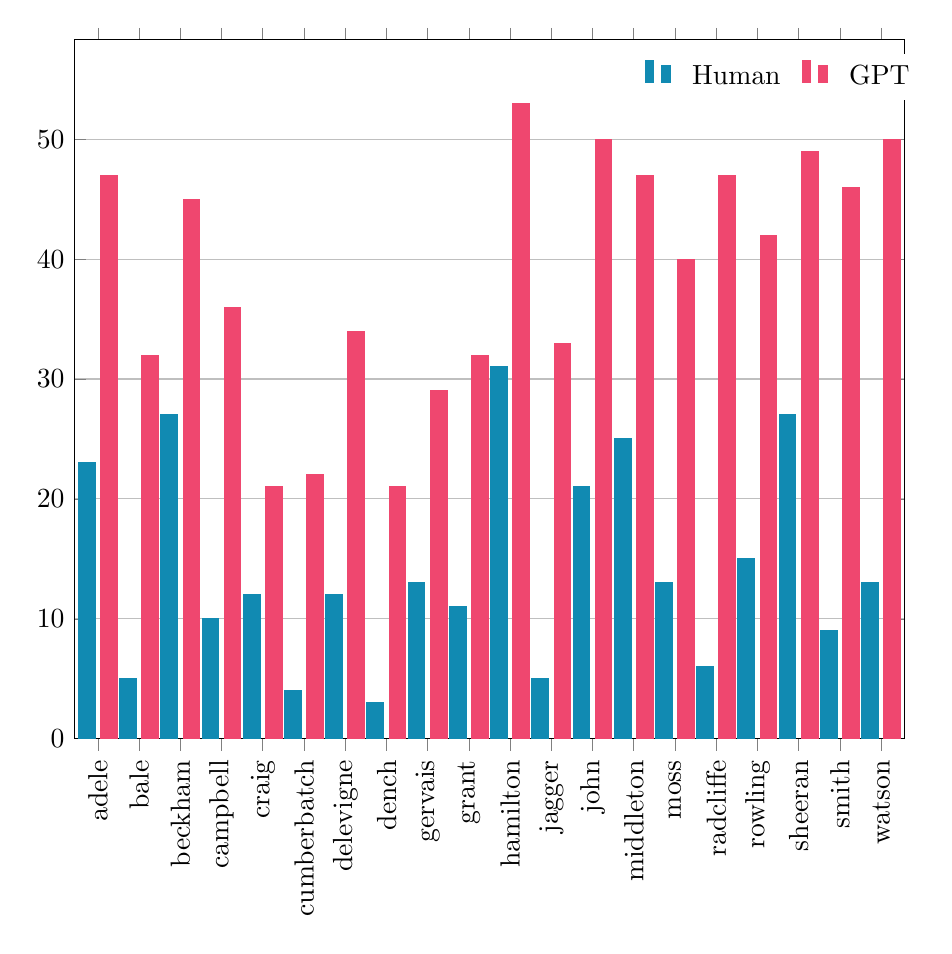
\begin{tikzpicture}  
\begin{axis}  
[  
    ybar,  
    width=\textwidth,
    enlarge x limits=0.03,
    ymin=0,ymajorgrids = true,
    xticklabels={adele,bale,beckham,campbell,craig,cumberbatch,delevigne,dench,gervais,grant,hamilton,jagger,john,middleton,moss,radcliffe,rowling,sheeran,smith,watson},
    bar width=6pt,
    % ylabel={Successful deanonymisation \%}, 
    xtick=data,   
    legend style={draw=none,at={(0.5,1.07)},anchor=north,column sep=0.2cm},legend columns=-1,
    xticklabel style={rotate=90},legend columns=-1,
        legend style={draw=none,at={(0.85,0.98)},anchor=north},
    ]  
    % human
\addplot [col2,fill=col2] coordinates {(0,23) (1,5) (2,27) (3,10) (4,12) (5,4) (6,12) (7,3) (8,13) (9,11) (10,31) (11,5) (12,21) (13,25) (14,13) (15,6) (16,15) (17,27) (18,9) (19,13)};  
\addplot [col1,fill=col1] coordinates {(0,47) (1,32) (2,45) (3,36) (4,21) (5,22) (6,34) (7,21) (8,29) (9,32) (10,53) (11,33) (12,50) (13,47) (14,40) (15,47) (16,42) (17,49) (18,46) (19,50) };  
\legend{Human,GPT}
\end{axis}  
\end{tikzpicture}
\caption{Successfully deanonymised text per celebrity by GPT and humans.}
\label{fig:anon_exp}
\end{figure}

\begin{figure}[th]
    \centering
    \includegraphics[width=\textwidth]{images/misclass.pdf}
    \caption{Misclassification in the deanonymisation.}
    \label{fig:misclass}
\end{figure}

\subsection{Anonymisation}
In the second experiment, we explore the extent to which GPT can effectively anonymise texts, as well as identify leakage of information that could lead to deanonymisation. First, we compare the GPT anonymisation efficacy to the one of Textwash. To this, we ask GPT to anonymise all 1080 of the original texts studied in the previous experiment using prompt~\ref{prompt:anon}, and for the produced outputs, we repeat the motivated intruder test \cite{mackey2016anonymisation}. Note that we frame the text anonymisation as a zero-shot task without providing specific examples of what needs to be redacted in the original texts. An example of anonymised text produced by GPT is displayed in Table~\ref{tab:anon_gpt}. We note that the anonymised texts produced by GPT are more readable and semantically coherent than the ones typically produced by anonymisation tools, as the redacted information is not just replaced by a tag, but the surrounding text is rewritten to maintain continuity of meaning.

In total, GPT successfully deanonymised 738 texts (729 in the first attempt and 9 in the 2nd), resulting in a deanonymisation rate of 68.3\%, only 11.4\% lower than what we observed for the texts anonymised with Textwash. As such, we can assume that zero-shot anonymisation using LLMs, while slightly more successful than using a state-of-the-art purpose-built anonymiser, cannot be considered an effective counter-measure mitigating the threat scenario described in Section~\ref{sec:scenario}. Moreover, since the texts produced are largely altered compared to their originals, it is difficult to directly compare with the outputs of Textwash and evaluate the capacity of GPT to identify PII and sensitive words. 

To this end, we focus on the 784 texts that were successfully deanonymised in the first trial of the motivated intruder test, see previous section. We prompt GPT to report the most relevant excerpts in the original texts that provide identifying information regarding the described person; see Table~\ref{prompt:tokens}. Note that we explicitly requested JSON-formatted output from GPT to facilitate the process of matching the exact excerpts in the original texts, as well as comparing them with the entities redacted by Textwash and their tags. Finally, we remove the returned excerpts from the original texts and repeat the motivated intruder test.

\subsection{Evaluation}
In total, 459 out of the 784 person descriptions were deanonymised (58.54\%), which indicates that while text anonymisation can be substantially improved compared to the Textwash baseline (all of these texts were successfully deanonymised by GPT), there is still work that needs to be done to consider text anonymisation as an adequate mechanism for ensuring the privacy of text data in the era of LLMs. Next, to better understand the capacity of GPT to find identifying information, we perform a series of comparisons with the output of Textwash for the corresponding texts. 
%Notably, Textwash is based on supervised machine learning, leveraging pre-trained contextualised word representations provided by the underlying BERT language model. As such, much like the NER-based text anonymisation tools, the categories of redactable text data considered by Textwash comprise a pre-defined set of 11 possible tags, the annotations for which were provided by domain experts. The last tag comprises a meta-category which encapsulates the \textbf{potentially sensitive information} (PSI) concept introduced in \cite{kleinberg2022textwash}. Concretely, the PSI notion captures the full spectrum of textual information that could reveal an identity which cannot be attributed to a well-defined category of PII. This is made possible by leveraging the contextual awareness of its Transformer-based architecture \cite{liu2019roberta,xia2020bert}. 
To this end, we parse token by token the pairs of the original and anonymised by the Textwash texts and extract the tags of the redacted tokens, which we then compare with the ones returned by GPT to capture the subset of tokens returned by both methods and their categories. We plot the results in Figure~\ref{fig:terms}. 

Interestingly, the most prevalent tag returned by Textwash, PRONOUN, is largely absent from the GPT output (2365 vs 59 instances, respectively). This means that -against human intuition- redacting the pronouns has a negligible impact on the text anonymisation for an LLM. An exception to the latter is that GPT returned the ``they/them'' pronouns, commonly used for non-binary individuals (see Table~\ref{tab:gpt_tokens}), which Textwash does not capture.
For the other categories, we observe that the tokens returned by GPT are aligned with the tokens redacted by Textwash to a large extent ($>70\%$), further highlighting the capacity of LLMs to capture sensitive information from text, even under a zero-shot setting without task-specific training.
\begin{figure}[th]
\centering
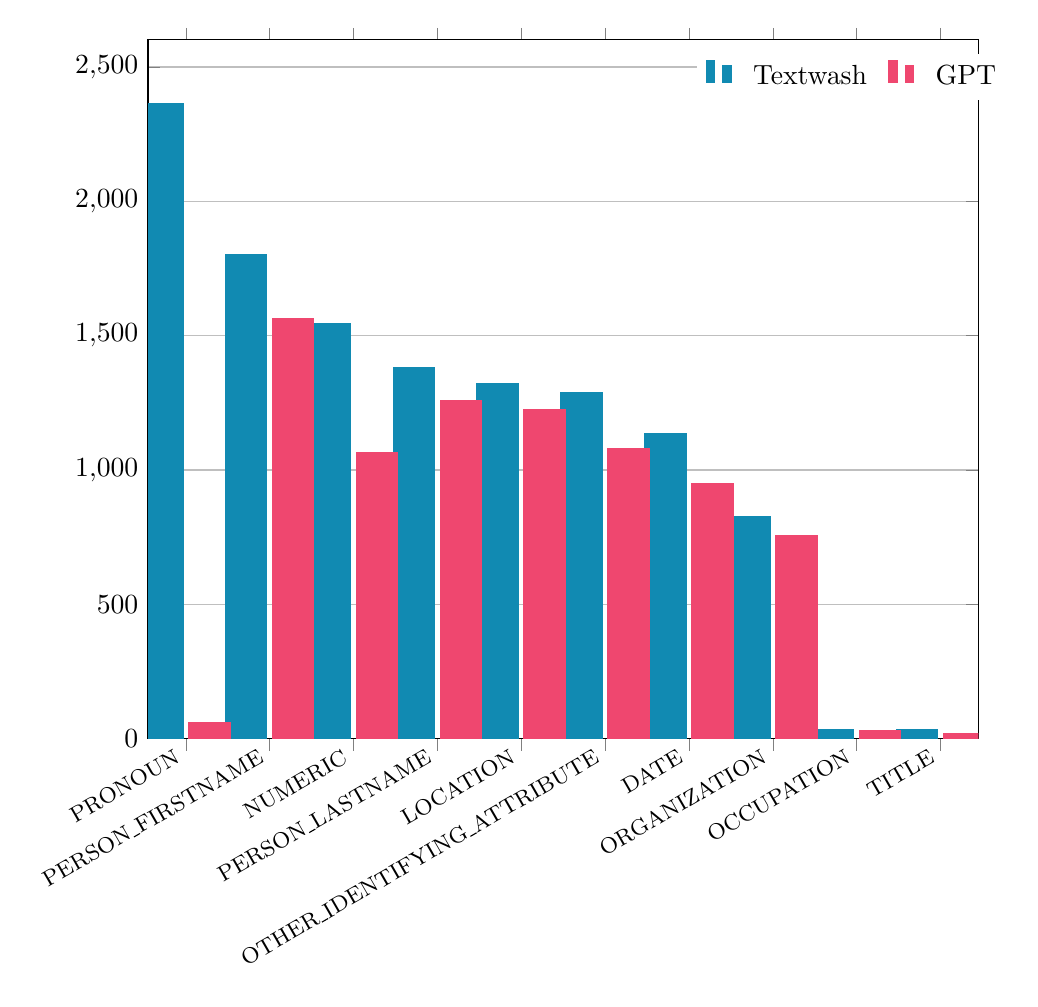
\begin{tikzpicture}  
\begin{axis}  
[  
    ybar,  
    width=\textwidth,
    enlarge x limits=0.05,
    ymin=0,ymajorgrids = true,
    xticklabels={PRONOUN, PERSON\_FIRSTNAME, NUMERIC, PERSON\_LASTNAME, LOCATION, OTHER\_IDENTIFYING\_ATTRIBUTE, DATE, ORGANIZATION, OCCUPATION, TITLE},
    bar width=15pt,
    xtick=data,   
    x tick label style={font=\footnotesize} ,
    legend style={draw=none,at={(0.5,1.07)},anchor=north,column sep=0.2cm},legend columns=-1,
    xticklabel style={rotate=30,anchor=east},legend columns=-1,
        legend style={draw=none,at={(0.85,0.98)},anchor=north},
    ]  
    % textwash
\addplot [col2,fill=col2] coordinates {(0,2365) (1,1802) (2,1544) (3,1383) (4,1321) (5,1287) (6,1134) (7,827) (8,33) (9,33)};  
% gpt
\addplot [col1,fill=col1] coordinates {(0,59) (1,1563) (2,1065) (3,1259) (4,1224) (5,1079) (6,949) (7,758) (8,30) (9,19)};  
\legend{Textwash,GPT}
\end{axis}  
\end{tikzpicture}
\caption{Removed terms.}
\label{fig:terms}
\end{figure}

Next, we measure the differences in text anonymisation based on the tokens that each method removed. We particularly focus on the proportion of anonymised text identified by Kleinberg et al. as the only statistically significant variable correlated with the deanonymisation success in their motivated intruder test. Concretely, this metric is calculated as \[P_{anon} = 1 - \frac{ntok_{original}-ntok_{anonymised}}{ntok_{original}}\], where
$ntok$ denotes the number of tokens in each text (original or anonymised). To this end, in Figure \ref{fig:prop_anon_txt}, we plot the cumulative distribution functions (CDFs) of $P_{anon}(TW)$ (Textwash) and $P_{anon}(GPT)$ w.r.t the success our GPT motivated intruder test. We observe that in both cases of successful and failed de-anonymisation, $P_{anon}(TW)$ acts as an upper bound to $P_{anon}(GPT)$, meaning that GPT is consistently more efficient than Textwash in terms of the proportion of tokens per text identified as sensitive. Expectedly, for both methods, the $P_{anon}$ of the texts that were successfully deanonymised by GPT is lower than the cases where the motivated intruder test failed. The biggest difference is observed for $P_{anon}(GPT)$, around 5\% between the instances of successful and unsuccessful de-anonymisation. 

The superior performance of GPT to capture sensitive tokens motivated us to assess the impact on text anonymisation of the tokens exclusively returned by GPT compared to those captured by both methods. For this, we calculate the fraction of tokens (per text) as follows. Let $\mathcal{T}_{TW}$ denote the set of tokens redacted by Textwash and $\mathcal{T}_{GPT}$ denote the set of sensitive tokens returned by GPT. Then, the fraction of identified tokens that are attributed to Textwash is:  
\[\mathcal{F}(TW) = \frac{|\mathcal{T}_{TW}|}{|\mathcal{T}_{TW} \cup \mathcal{T}_{GPT}|}\]
Similarly, the fraction of tokens that are exclusively attributed to GPT is:
\[\mathcal{F}(GPT) = \frac{|\mathcal{T}_{GPT} \setminus \mathcal{T}_{TW}|}{|\mathcal{T}_{TW} \cup \mathcal{T}_{GPT}|}\]
We plot the CDFs of these fractions for the texts w.r.t the success of the GPT-motivated intruder test in Figure \ref{fig:prop_anon_tok}. We observe that where the test failed (anonymisation was successful), $\mathcal{F}(GPT)$ is consistently higher than $\mathcal{F}(TW)$, by a margin of $20\%$ on average (for the cases where the identification test failed, on average the 59.5\% of total sensitive tokens where exclusively identified by GPT, while Textwash captured the 40.5\%). For the cases where the test succeeded, the difference between $\mathcal{F}(GPT)$ and $\mathcal{F}(TW)$ is considerably lower, with average values of 47.2\% and 52.3\% for Textwash and GPT, respectively. These observations further prove the capacity of GPT to capture salient tokens encompassing sensitive information (PSI), surpassing even the results of state-of-the-art anonymisation tools like Textwash, specifically fine-tuned for this task. To better explore this, in Table~\ref{tab:gpt_tokens}, we present the top terms lemmatised using spaCy\footnote{\url{https://spacy.io}} and bi-grams that GPT exclusively captured. Indeed, their majority comprises specific features capable of revealing the identity of each individual, as well as false negatives for Textwash, such as surname. Similar tokens were also identified by Kleinberg et al. as being responsible for the information leakage leading to successful deanonymisation (by humans). Nevertheless, we observe the existence of terms that are rather generic but provided the context they appear in, their removal obstructs the overall understanding of a reader.


\begin{figure}[th]
    \centering
    \includegraphics[width=.7\textwidth]{images/prop_rem_txt.pdf}
    \caption{Proportion of text removed by each method for the cases where the motivated intruder test of person identification succeeded or failed.}
    \label{fig:prop_anon_txt}
\end{figure}


\begin{figure}[th]
    \centering
    \includegraphics[width=.7\textwidth]{images/prop_anon_tok.pdf}
    \caption{Fractions of the sensitive tokens exclusively captured by each method for the cases where the motivated intruder test of person identification succeeded or failed (only for the 784 descriptions successfully deanonymised in the first trial of the motivated intruder test).}
    \label{fig:prop_anon_tok}
\end{figure}


\begin{table}[th]
    \centering
    \footnotesize
    \rowcolors{2}{gray!15}{white}
\begin{tabular}{lp{5in}}
\toprule
     \textbf{Celebrity} &                                                                                                                                                                                \textbf{Sensitive terms exclusively captured by GPT} \\
\midrule
       elton john &                                             singer (40), songwriter (21), marry (17), pianist (17), composer (17), award (14), song (13), piano (11), musician (9), film (8), record (8), child (7) \\
    jk rowling &                                author (22), book (15), film (10), female (10), writer (8), charity (6), benefit (6), twitter (6), billionaire (5), best\_selling (4), publisher (4), controversy (4) \\
       christian bale &                                                          actor (22), marry (10), award (8), batman (7), role (6), academy (4), dark (4), film (4), movie (3), act (3), weight (3), golden\_globe (3) \\
      sam smith &                                    singer (39), award (24), songwriter (22), gay (18), non\_binary (18), they (12), they\_them (11), song (11), genderqueer (10), music (10), pronoun (9), single (8) \\
  daniel radcliffe &                                                  actor (24), film (12), franchise (7), movie (5), stage (5), theatre (4), young (4), act (4), play (3), charity (3), accolade (3), relationship (3) \\
  kate middleton &                        child (13), marry (13), prince (12), charity (10), mental\_health (10), university (7), royal\_family (7), sport (6), charity\_work (6), art\_history (5), mother (5), royal (5) \\
   naomi campbell &                                   model (24), supermodel (19), singer (11), actress (8), father (6), businesswoman (5), dancer (5), rehab (5), assault (5), singe (4), music\_videos (4), mother (4) \\
     emma watson & actress (29), activist (14), women\_rights (13), model (13), feminist (11), harry\_potter (8), gender\_equality (6), film (6), woman (6), un\_women\_goodwill\_ambassador (5), ambassador (5), potter (4) \\
      judi dench &                                                            actress (20), film (15), award (11), marry (5), academy (5), husband (4), bafta (4), year (4), best (4), play (4), support (4), love (3) \\
      adele &                                      singer (31), award (20), album (18), songwriter (16), grammy (13), child (13), marry (11), divorced (9), voice (9), sell (9), someone\_like\_you (8), artist (7) \\
    david beckham &                          footballer (21), marry (15), model (9), retire (9), tattoo (8), professional (8), football\_player (8), football (7), beckham (7), league (6), posh\_spice (5), co\_owner (5) \\
 cara delevingne &                                                  model (37), actress (23), singer (15), eyebrow (11), sister (9), bisexual (8), act (7), guitar (7), film (7), drum (6), fashion (6), pansexual (5) \\
   lewis hamilton &                driver (16), race (15), racing\_driver (11), win (10), podium\_finishes (9), vegan (8), racism (8), black\_driver (7), championship (7), father (7), motorsport (6), pole\_positions (6) \\
       kate moss &               supermodel (24), model (22), daughter (15), drug\_use (8), businesswoman (7), party\_lifestyle (7), drug\_allegations (7), drug (7), fashion (7), heroin\_chic (6), moss (4), catwalk (4) \\
      daniel craig &          actor (11), marry (8), film (6), play (3), international\_fame (3), the\_girl\_with\_the\_dragon\_tattoo (3), knives\_out (3), stage (2), action (2), british (2), casino\_royale (2), spectre (2) \\
    ricky gervais &                                          comedian (18), actor (17), writer (13), director (9), award (9), write (8), the\_office (8), podcast (7), producer (6), pop\_star (6), golden (6), globe (6) \\
      hugh grant &                                  actor (24), romantic\_comedies (9), film (8), bafta (7), golden\_globe (7), about\_boy (5), golden (5), globe (5), child (5), funny (4), marry (4), love\_actually (4) \\
     mick jagger &                                        singer (20), songwriter (13), band (11), actor (10), knight (8), relationship (7), film (7), child (7), lead\_singer (6), producer (6), popular (6), roll (6) \\
    ed sheeran &                            singer (19), marry (19), guitar (16), musician (14), singer\_songwriter (13), song (12), actor (11), songwriter (11), ginger\_hair (10), album (10), award (8), artist (7) \\
benedict cumberbatch &                                                              actor (18), award (11), emmy (5), marry (5), cbe (4), academy (4), bbc (4), screen (4), sherlock (3), tall (3), bafta (3), theatre (3) \\
\bottomrule
\end{tabular}
    \caption{Most frequent terms (1- and 2-grams) appearing in person descriptions only captured by GPT $(\in \mathcal{T}_{GPT} \setminus \mathcal{T}_{TW})$.}
    \label{tab:gpt_tokens}
\end{table}

\subsection{Comparison with existing work}
Recently, some researchers have started investigating the potential leakage of private sensitive information from language models.  Lehman et al. \cite{lehman2021does} considered the case of BERT, leaking privacy data. The authors conclude that while some associations can be made, they are not enough to be considered a threat. Note that in one of their attacks, the names of patients were kept in the training samples, yet the associations did not significantly increase.

Brown et al. \cite{brown2022does} acknowledge the potential risks of large language models leaking private information and therefore highlight the need for training the models with data intended to be public and not simply publicly available data. The latter is aligned with Zimmer's approach \cite{zimmer2010but}, as people who may have published something do not make it public for every possible use and cannot be aware of the implications that it could have when correlated with other information. More importantly, Brown et al. stress that traditional and effective methods like differential privacy do not apply to such language models.
Undoubtedly, the closest work to ours is that of Lukas et al. \cite{lukas2023analyzing}, who used GPT-2 on three datasets and successfully managed to extract PIIs from anonymised texts. Nevertheless, the attacks refer to generic PIIs and not full deanonymisation, and their threat scenario is completely different to ours. Moreover, there is no actual comparison of what a human could achieve.

Based on the above, we claim that our work is the first one to leverage LLMs to fully deanonymise a dataset of anonymised texts with such accuracy and illustrate the risks implied by the use of fine-tuned LLMs. Moreover, the comparison with human capacity as well as the identification of which pieces of information may lead to the deanonymisation of individuals has not been performed in the related literature. Finally, we should note that using other prompts, the deanonymisation not only of the person but of all other redacted information is revealed, see Figure \ref{tab:deanon_gpt}. As it can be observed, GPT, correctly replaced 20 redacted tags out of the total 23. Notably, the three mistakes are one for the replacement of a pronoun with the name and the two advertised companies which in the original text were Vogue and Chanel. However, a simple web search shows that the result is correct as she has advertised the products of both Burberry and Lan\^{o}me. Therefore, the misses cannot be claimed as being wrong. 

The latter implies that even when the deanonymisation might not have been successful, other PIIs could have been extracted; however, they were not considered in this work and are left for future work. Therefore, a comparison in terms of the percentage of extracted PIIs to \cite{lukas2023analyzing} would clearly show that this approach is far more efficient. Indeed, our claims are justified can be justified by the misclassifications of Figure \ref{fig:misclass} where one can observe obvious extraction of some PIIs (e.g., ethnicity, age group, gender) when the deanonymisation task failed.

\begin{table}[th]

\centering
\begin{tabular}{|p{\textwidth}|}
    \hline
    \cellcolor{col2!10}\textbf{System:} You are an efficient assistant. Find which celebrity matches the following description and match the missing information\\
    \hline \textbf{User:} PERSON\_FIRSTNAME\_1 PERSON\_LASTNAME\_2 is a NUMERIC\_4 year old actress, born in LOCATION\_2 but raised in the LOCATION\_1. PRONOUN is most famously known for playing PERSON\_FIRSTNAME\_2 PERSON\_LASTNAME\_1 in the OTHER\_IDENTIFYING\_ATTRIBUTE\_2 franchise. PRONOUN played this role for NUMERIC\_3 years and was it was actually PRONOUN first professional role of PRONOUN acting career. Another note-worthy performance from PERSON\_FIRSTNAME\_1 PERSON\_LASTNAME\_2 was PRONOUN role in the DATE\_1 live action OTHER\_IDENTIFYING\_ATTRIBUTE\_1, where PRONOUN played the main character PERSON\_FIRSTNAME\_3. PRONOUN is also very present in the fashion world, becoming a model at a young age and working with companies such as ORGANIZATION\_1 and ORGANIZATION\_2. More importantly, PRONOUN is very involved in activism and is a very outspoken feminist.\\   
    \hline \textbf{Assistant:} \mybox{col4}{Emma} \mybox{col4}{Watson} is a \mybox{col4}{31} year old actress, born in \mybox{col4}{Paris} but raised in the \mybox{col4}{UK}. She is most famously known for playing \mybox{col4}{Hermione} \mybox{col4}{Granger} in the \mybox{col4}{Harry Potter} franchise. \mybox{col4}{Emma} played this role for \mybox{col4}{10} years and it was actually \mybox{col4}{her} first professional role of \mybox{col4}{her} acting career. Another note-worthy performance from \mybox{col4}{Emma} \mybox{col4}{Watson} was \mybox{col4}{her} role in the \mybox{col4}{2017} live action \mybox{col4}{Beauty and the Beast}, where \mybox{col4}{she} played the main character \mybox{col4}{Belle}. \mybox{col2}{Emma} is also very present in the fashion world, becoming a model at a young age and working with companies such as \mybox{col1}{Burberry} and \mybox{col1}{Lan\^{o}me}. More importantly, \mybox{col4}{she} is very involved in activism and is a very outspoken feminist.\\
   
    \hline
\end{tabular}
\caption{An example of a fully deanonymised text produced by GPT.}
\label{tab:deanon_gpt}
\end{table}



\section{Conclusions}
Our work puts more water to the mill in the discussion of the ethical use of AI. As common practice shows, companies will exploit the data that they have legally and ethically collected from their clients and the internet to infer more data for them. The reason is that this abundance of information can be used to personalise their products and services. As a result, they increase their quality, market penetration, and of course, their income. In fact, many companies are already touting that they can enable such functionalities while the cost for creating a trained GPT alternative, e.g. BLOOM\footnote{\url{https://huggingface.co/bigscience/bloom-7b1}} is in the scale of \$7 million, and the cost is expected to significantly drop\footnote{\url{https://techcrunch.com/2022/07/12/a-year-in-the-making-bigsciences-ai-language-model-is-finally-available}}.  In this regard, we believe that it is only a matter of time before organisations start using LLMs on their documents and realise that this way, not only can they get more visibility about their customers, but they can also deanonymise documents revealing information that would be impossible for them to do so. 

As illustrated through our experiments, the use of LLMs for document deanonymisation can have a devastating impact. In fact, using an off-the-shelf commercial solution, GPT, which is not explicitly trained on such data nor for this goal, exhibited remarkable results in document deanonymisation of celebrities by outperforming humans almost three times. We argue that the above justifies the need to consider LLMs a significant threat in the era of big data and artificial intelligence. Moreover, the results challenge what we perceive as identifying information as humans and what a machine does. While important for us features, e.g. pronouns are disregarded, even minor linguistic or knowledge hints can lead to complete deanonymisation. 


While we acknowledge that this threat might have always been in the back of the mind of several researchers when discussing privacy violations and possible abuse from artificial intelligence, the misuse of big data and background knowledge, this is the first work that practically illustrates this attack over anonymised texts. Indeed, the comparison of the human capacity to anonymise celebrities by synthesising the information from relatively short anonymised texts is by far exceeded by LLMs, even if they were not trained explicitly for this task. Thus, one can safely assume that if the texts were longer, the results of the LLM would be significantly better as more correlations could be extracted. We argue that the above not only validates how realistic our threat scenario is but also shows that the threat can be significantly augmented as visual data can be processed alongside text \cite{suris2023vipergpt}. The above contrasts to \cite{huang2022large}, yet we attribute this change to the stronger association of the new models. Note that Huang et al. \cite{huang2022large} attribute the results of the deanonymisations to memorisation due to the low association capabilities of the LLM they used. Yet, our results indicate far more advanced association capabilities and a significantly higher risk.

Further to merely considering LLMs a part of the problem, we used them for document anonymisation. Our revised document anonymisation pipeline improves the current state; however, there is still much room for improvement as the results might be improved, but not enough to consider the users secure. We believe that a promising direction would be to consider the adversarial model so that the text contains implicit information in the form of words to trick the LLM into providing the wrong answer in case of a deanonymisation task. This way, the privacy of individuals would be protected since the result of the LLM would be considered valid yet it would actually be wrong. To this end, we plan in future work to study the confidence level of the responses of LLMs and how we can introduce small yet hard-to-detect text fragments to bias the results of LLMs in the case of deanonymisation attacks. 

\section*{Acknowledgments}
This work was supported by the European Commission under the Horizon 2020 Programme (H2020), as part of the project HEROES (\url{https://heroes-fct.eu/}) (Grant Agreement no. 101021801) and under the Horizon Europe Programme, as part of the project LAZARUS (\url{https://lazarus-he.eu/}) (Grant Agreement no. 101070303).

The content of this article does not reflect the official opinion of the European Union. Responsibility for the information and views expressed therein lies entirely with the authors.

\begin{thebibliography}{10}

\bibitem{brants2007large}
Thorsten Brants, Ashok~C. Popat, Peng Xu, Franz~Josef Och, and Jeffrey Dean.
\newblock Large language models in machine translation.
\newblock In Jason Eisner, editor, {\em EMNLP-CoNLL 2007, Proceedings of the
  2007 Joint Conference on Empirical Methods in Natural Language Processing and
  Computational Natural Language Learning, June 28-30, 2007, Prague, Czech
  Republic}, pages 858--867. {ACL}, 2007.

\bibitem{brown2022does}
Hannah Brown, Katherine Lee, Fatemehsadat Mireshghallah, Reza Shokri, and
  Florian Tram{\`e}r.
\newblock What does it mean for a language model to preserve privacy?
\newblock In {\em 2022 ACM Conference on Fairness, Accountability, and
  Transparency}, pages 2280--2292, 2022.

\bibitem{brown2020language}
Tom Brown, Benjamin Mann, Nick Ryder, Melanie Subbiah, Jared~D Kaplan, Prafulla
  Dhariwal, Arvind Neelakantan, Pranav Shyam, Girish Sastry, Amanda Askell,
  et~al.
\newblock Language models are few-shot learners.
\newblock {\em Advances in neural information processing systems},
  33:1877--1901, 2020.

\bibitem{brundage2020toward}
Miles Brundage, Shahar Avin, Jasmine Wang, Haydn Belfield, Gretchen Krueger,
  Gillian Hadfield, Heidy Khlaaf, Jingying Yang, Helen Toner, Ruth Fong, et~al.
\newblock Toward trustworthy ai development: mechanisms for supporting
  verifiable claims.
\newblock {\em arXiv preprint arXiv:2004.07213}, 2020.

\bibitem{dernoncourt2017identification}
Franck Dernoncourt, Ji~Young Lee, Ozlem Uzuner, and Peter Szolovits.
\newblock De-identification of patient notes with recurrent neural networks.
\newblock {\em Journal of the American Medical Informatics Association},
  24(3):596--606, 2017.

\bibitem{DevlinCLT19}
Jacob Devlin, Ming{-}Wei Chang, Kenton Lee, and Kristina Toutanova.
\newblock {BERT:} pre-training of deep bidirectional transformers for language
  understanding.
\newblock In Jill Burstein, Christy Doran, and Thamar Solorio, editors, {\em
  Proceedings of the 2019 Conference of the North American Chapter of the
  Association for Computational Linguistics: Human Language Technologies,
  {NAACL-HLT} 2019, Minneapolis, MN, USA, June 2-7, 2019, Volume 1 (Long and
  Short Papers)}, pages 4171--4186. Association for Computational Linguistics,
  2019.

\bibitem{aiact}
{European Commission}.
\newblock {Proposal for a REGULATION OF THE EUROPEAN PARLIAMENT AND OF THE
  COUNCIL LAYING DOWN HARMONISED RULES ON ARTIFICIAL INTELLIGENCE (ARTIFICIAL
  INTELLIGENCE ACT) AND AMENDING CERTAIN UNION LEGISLATIVE ACTS}.
\newblock
  \url{https://eur-lex.europa.eu/legal-content/EN/TXT/?uri=celex\%3A52021PC0206},
  2021.

\bibitem{gdpr}
{Regulation (EU) 2016/679 of the European Parliament and of the Council of 27
  April 2016 on the protection of natural persons with regard to the processing
  of personal data and on the free movement of such data, and repealing
  Directive 95/46/EC (General Data Protection Regulation), Official Journal of
  the European Union, Vol. L119 (4 May 2016), pp. 1-88}, 2016.

\bibitem{978-3-030-00202-2_24}
Fadi Hassan, Josep Domingo-Ferrer, and Jordi Soria-Comas.
\newblock Anonymization of unstructured data via named-entity recognition.
\newblock In Vicen{\c{c}} Torra, Yasuo Narukawa, Isabel Aguil{\'o}, and Manuel
  Gonz{\'a}lez-Hidalgo, editors, {\em Modeling Decisions for Artificial
  Intelligence}, pages 296--305, Cham, 2018. Springer International Publishing.

\bibitem{huang2022large}
Jie Huang, Hanyin Shao, and Kevin~Chen{-}Chuan Chang.
\newblock Are large pre-trained language models leaking your personal
  information?
\newblock In Yoav Goldberg, Zornitsa Kozareva, and Yue Zhang, editors, {\em
  Findings of the Association for Computational Linguistics: {EMNLP} 2022, Abu
  Dhabi, United Arab Emirates, December 7-11, 2022}, pages 2038--2047.
  Association for Computational Linguistics, 2022.

\bibitem{kleinberg2022textwash}
Bennett Kleinberg, Toby Davies, and Maximilian Mozes.
\newblock Textwash--automated open-source text anonymisation.
\newblock {\em arXiv preprint arXiv:2208.13081}, 2022.

\bibitem{kleinberg2017netanos}
Bennett Kleinberg and Maximilian Mozes.
\newblock Web-based text anonymization with node.js: Introducing {NETANOS}
  (named entity-based text anonymization for open science).
\newblock {\em J. Open Source Softw.}, 2(14):293, 2017.

\bibitem{lehman2021does}
Eric Lehman, Sarthak Jain, Karl Pichotta, Yoav Goldberg, and Byron~C. Wallace.
\newblock Does {BERT} pretrained on clinical notes reveal sensitive data?
\newblock In Kristina Toutanova, Anna Rumshisky, Luke Zettlemoyer, Dilek
  Hakkani{-}T{\"{u}}r, Iz~Beltagy, Steven Bethard, Ryan Cotterell, Tanmoy
  Chakraborty, and Yichao Zhou, editors, {\em Proceedings of the 2021
  Conference of the North American Chapter of the Association for Computational
  Linguistics: Human Language Technologies, {NAACL-HLT} 2021, Online, June
  6-11, 2021}, pages 946--959. Association for Computational Linguistics, 2021.

\bibitem{lison2021anonymisation}
Pierre Lison, Ildik{\'o} Pil{\'a}n, David S{\'a}nchez, Montserrat Batet, and
  Lilja {\O}vrelid.
\newblock Anonymisation models for text data: State of the art, challenges and
  future directions.
\newblock In {\em Proceedings of the 59th Annual Meeting of the Association for
  Computational Linguistics and the 11th International Joint Conference on
  Natural Language Processing (Volume 1: Long Papers)}, pages 4188--4203, 2021.

\bibitem{liu2019roberta}
Yinhan Liu, Myle Ott, Naman Goyal, Jingfei Du, Mandar Joshi, Danqi Chen, Omer
  Levy, Mike Lewis, Luke Zettlemoyer, and Veselin Stoyanov.
\newblock Roberta: A robustly optimized bert pretraining approach.
\newblock {\em arXiv preprint arXiv:1907.11692}, 2019.

\bibitem{LIU2017S34}
Zengjian Liu, Buzhou Tang, Xiaolong Wang, and Qingcai Chen.
\newblock De-identification of clinical notes via recurrent neural network and
  conditional random field.
\newblock {\em Journal of Biomedical Informatics}, 75:S34--S42, 2017.
\newblock Supplement: A Natural Language Processing Challenge for Clinical
  Records: Research Domains Criteria (RDoC) for Psychiatry.

\bibitem{lukas2023analyzing}
Nils Lukas, Ahmed Salem, Robert Sim, Shruti Tople, Lukas Wutschitz, and
  Santiago~Zanella B{\'{e}}guelin.
\newblock Analyzing leakage of personally identifiable information in language
  models.
\newblock {\em CoRR}, abs/2302.00539, 2023.

\bibitem{mackey2016anonymisation}
Elaine Mackey, Mark Elliot, and Kieron O’Hara.
\newblock {\em The anonymisation decision-making framework}.
\newblock UKAN publications, 2016.

\bibitem{mamede2016automated}
Nuno Mamede, Jorge Baptista, and Francisco Dias.
\newblock Automated anonymization of text documents.
\newblock In {\em 2016 IEEE congress on evolutionary computation (CEC)}, pages
  1287--1294. IEEE, 2016.

\bibitem{manning2014stanford}
Christopher~D Manning, Mihai Surdeanu, John Bauer, Jenny~Rose Finkel, Steven
  Bethard, and David McClosky.
\newblock The stanford corenlp natural language processing toolkit.
\newblock In {\em Proceedings of 52nd annual meeting of the association for
  computational linguistics: system demonstrations}, pages 55--60, 2014.

\bibitem{meystre2010automatic}
Stephane~M Meystre, F~Jeffrey Friedlin, Brett~R South, Shuying Shen, and
  Matthew~H Samore.
\newblock Automatic de-identification of textual documents in the electronic
  health record: a review of recent research.
\newblock {\em BMC medical research methodology}, 10(1):1--16, 2010.

\bibitem{narayanan2010myths}
Arvind Narayanan and Vitaly Shmatikov.
\newblock Myths and fallacies of" personally identifiable information".
\newblock {\em Communications of the ACM}, 53(6):24--26, 2010.

\bibitem{neamatullah2008automated}
Ishna Neamatullah, Margaret~M Douglass, Li-Wei~H Lehman, Andrew Reisner,
  Mauricio Villarroel, William~J Long, Peter Szolovits, George~B Moody, Roger~G
  Mark, and Gari~D Clifford.
\newblock Automated de-identification of free-text medical records.
\newblock {\em BMC medical informatics and decision making}, 8(1):1--17, 2008.

\bibitem{ouyang2022training}
Long Ouyang, Jeff Wu, Xu~Jiang, Diogo Almeida, Carroll~L Wainwright, Pamela
  Mishkin, Chong Zhang, Sandhini Agarwal, Katarina Slama, Alex Ray, et~al.
\newblock Training language models to follow instructions with human feedback.
\newblock {\em arXiv preprint arXiv:2203.02155}, 2022.

\bibitem{ruch2000medical}
Patrick Ruch, Robert~H Baud, Anne-Marie Rassinoux, Pierrette Bouillon, and
  Gilbert Robert.
\newblock Medical document anonymization with a semantic lexicon.
\newblock In {\em Proceedings of the AMIA Symposium}, page 729. American
  Medical Informatics Association, 2000.

\bibitem{samaratiyprotecting}
Pierangela Samaratiy and Latanya Sweeney.
\newblock Protecting privacy when disclosing information: k-anonymity and its
  enforcement through generalization and suppression, 1998.

\bibitem{sanchez2012detecting}
David S{\'a}nchez, Montserrat Batet, and Alexandre Viejo.
\newblock Detecting sensitive information from textual documents: an
  information-theoretic approach.
\newblock In {\em Modeling Decisions for Artificial Intelligence: 9th
  International Conference, MDAI 2012, Girona, Catalonia, Spain, November
  21-23, 2012. Proceedings 9}, pages 173--184. Springer, 2012.

\bibitem{sanchez2014utility}
David S{\'a}nchez, Montserrat Batet, and Alexandre Viejo.
\newblock Utility-preserving privacy protection of textual healthcare
  documents.
\newblock {\em Journal of biomedical informatics}, 52:189--198, 2014.

\bibitem{selbst2020negligence}
Andrew~D Selbst.
\newblock Negligence and ai's human users.
\newblock {\em BUL Rev.}, 100:1315, 2020.

\bibitem{smith2020artificial}
Helen Smith and Kit Fotheringham.
\newblock Artificial intelligence in clinical decision-making: Rethinking
  liability.
\newblock {\em Medical Law International}, 20(2):131--154, 2020.

\bibitem{suris2023vipergpt}
D{\'{\i}}dac Sur{\'{\i}}s, Sachit Menon, and Carl Vondrick.
\newblock Vipergpt: Visual inference via python execution for reasoning.
\newblock {\em CoRR}, abs/2303.08128, 2023.

\bibitem{sweeney1996replacing}
Latanya Sweeney.
\newblock Replacing personally-identifying information in medical records, the
  scrub system.
\newblock In {\em Proceedings of the AMIA annual fall symposium}, page 333.
  American Medical Informatics Association, 1996.

\bibitem{6410029}
David Sánchez, Montserrat Batet, and Alexandre Viejo.
\newblock Automatic general-purpose sanitization of textual documents.
\newblock {\em IEEE Transactions on Information Forensics and Security},
  8(6):853--862, 2013.

\bibitem{vaswani2007attention}
Ashish Vaswani, Noam Shazeer, Niki Parmar, Jakob Uszkoreit, Llion Jones,
  Aidan~N. Gomez, Lukasz Kaiser, and Illia Polosukhin.
\newblock Attention is all you need.
\newblock In Isabelle Guyon, Ulrike von Luxburg, Samy Bengio, Hanna~M. Wallach,
  Rob Fergus, S.~V.~N. Vishwanathan, and Roman Garnett, editors, {\em Advances
  in Neural Information Processing Systems 30: Annual Conference on Neural
  Information Processing Systems 2017, December 4-9, 2017, Long Beach, CA,
  {USA}}, pages 5998--6008, 2017.

\bibitem{xia2020bert}
Patrick Xia, Shijie Wu, and Benjamin Van~Durme.
\newblock Which* bert? a survey organizing contextualized encoders.
\newblock {\em arXiv preprint arXiv:2010.00854}, 2020.

\bibitem{zigomitros2020survey}
Athanasios Zigomitros, Fran Casino, Agusti Solanas, and Constantinos Patsakis.
\newblock A survey on privacy properties for data publishing of relational
  data.
\newblock {\em IEEE Access}, 8:51071--51099, 2020.

\bibitem{zimmer2010but}
Michael Zimmer.
\newblock "but the data is already public": on the ethics of research in
  facebook.
\newblock {\em Ethics and information technology}, 12:313--325, 2010.

\bibitem{UZUNER200813}
Özlem Uzuner, Tawanda~C. Sibanda, Yuan Luo, and Peter Szolovits.
\newblock A de-identifier for medical discharge summaries.
\newblock {\em Artificial Intelligence in Medicine}, 42(1):13--35, 2008.

\end{thebibliography}


\end{document}
